\subsection{Simulation results} \label{sec:fbl_sim}
The implemented control law was tested on a trajectory tracking task. To complete the task, the helicopter is required to perform, cyclically with period $T = \qty{100}{\second}$, an helical trajectory for $\qty{70}{\second}$ and then to come back to the origin in the remaining $\qty{30}{\second}$, while keeping the yaw angle to zero, i.e.
\begin{align}
    &P^d=\begin{cases*}
        \begin{bmatrix}
            r\cdot cos(\frac{t}{d}) \\ r\cdot sin(\frac{t}{d})\\ 1+\frac{t}{k}
        \end{bmatrix} \quad &if $t$ \% 50 $<$ 30 \\
        \begin{bmatrix}
            0 \\ 0 \\ 0
         \end{bmatrix} \quad &else
    \end{cases*} \label{eq:pos_ref}\\
    &W^d=0 \label{eq:yaw_ref}
\end{align}

\noindent with $r=\qty{5}{\meter}$ radius of the helix, $d=5$ a scaling factor regulating the speed of the $(x,y)$ plane and $k=10$ a scaling factor regulating the rate of climb. The symbol $\%$ stands for remainder after division. \\
Moreover, the initial position of the robot belongs to the helical trajectory, while the initial attitude is null.

For the sake of realism, the control inputs to the system cannot range over an infinite span, but it is appropriate to constrain them to vary over limited intervals. More specifically, we impose the following constraints:

\begin{gather}
    \omega_u \in [0, 2800] \, \textit{rpm} \label{eq:omega_u_constraint} \\
    \omega_l \in [-2800, 0] \, \textit{rpm} \label{eq:omega_l_constraint} \\
    \alpha \in [-10, 10]^\circ \label{eq:alpha_constraint} \\
    \beta \in [-10, 10]^\circ \label{eq:beta_constraint}
\end{gather}

Figure \ref{fig:FL_trajectory} shows the comparison between the reference and the actual trajectory traversed by the robot. The tracking performance is outstanding as long as the error is small, but failure occurs in the instant that the error is too large, because of the explosion of the states governing the forced zero dynamics. We deduce that the system is extremely unrobust, so the control action is not sufficiently reliable.
\begin{figure}[H]
    \centering
    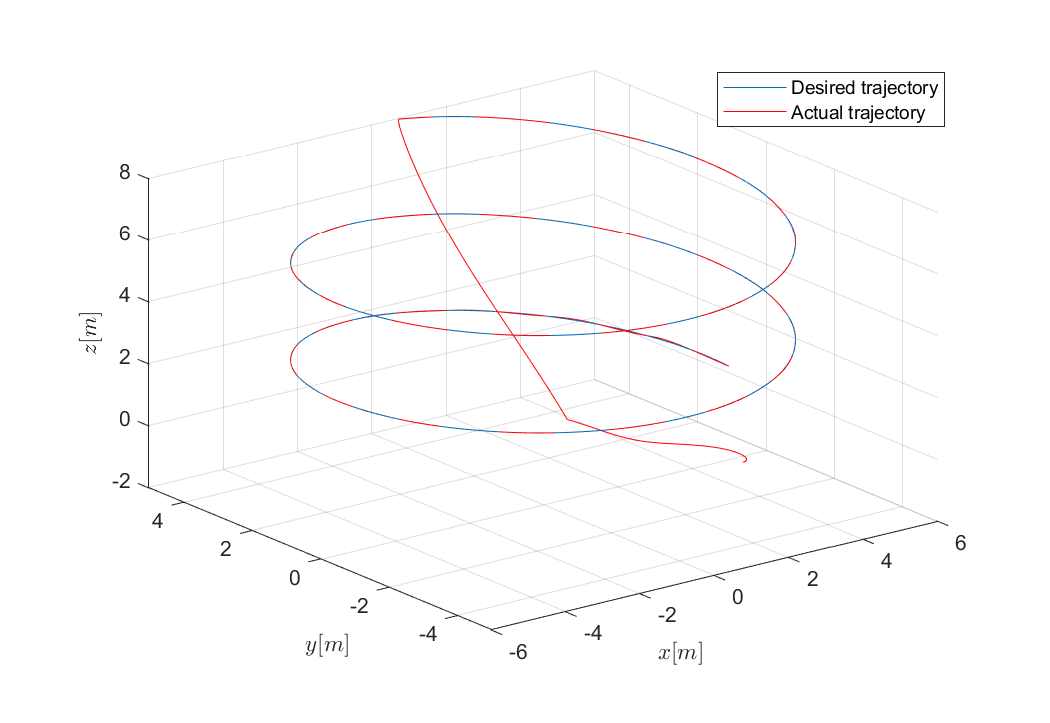
\includegraphics[scale=0.5]{figures/FL_trajectory}
    \caption{Trajectory tracking.}
    \label{fig:FL_trajectory}
\end{figure}
This phenomenon is also visible in Figure \ref{fig:FL_attitude}. Despite the pitch having, up to a certain point, an acceptable evolution, the roll exhibits noticeable fluctuations that induce Ingenuity to assume an unrealistic behavior. As an additional consequence, the small angles assumption of the previous signals is violated, leading to a significant error in the yaw angle, whose reference is not followed. Moreover, as in the previous graph, the abrupt change in the reference causes the bursting of the examined states.
\begin{figure}[H]
    \centering
    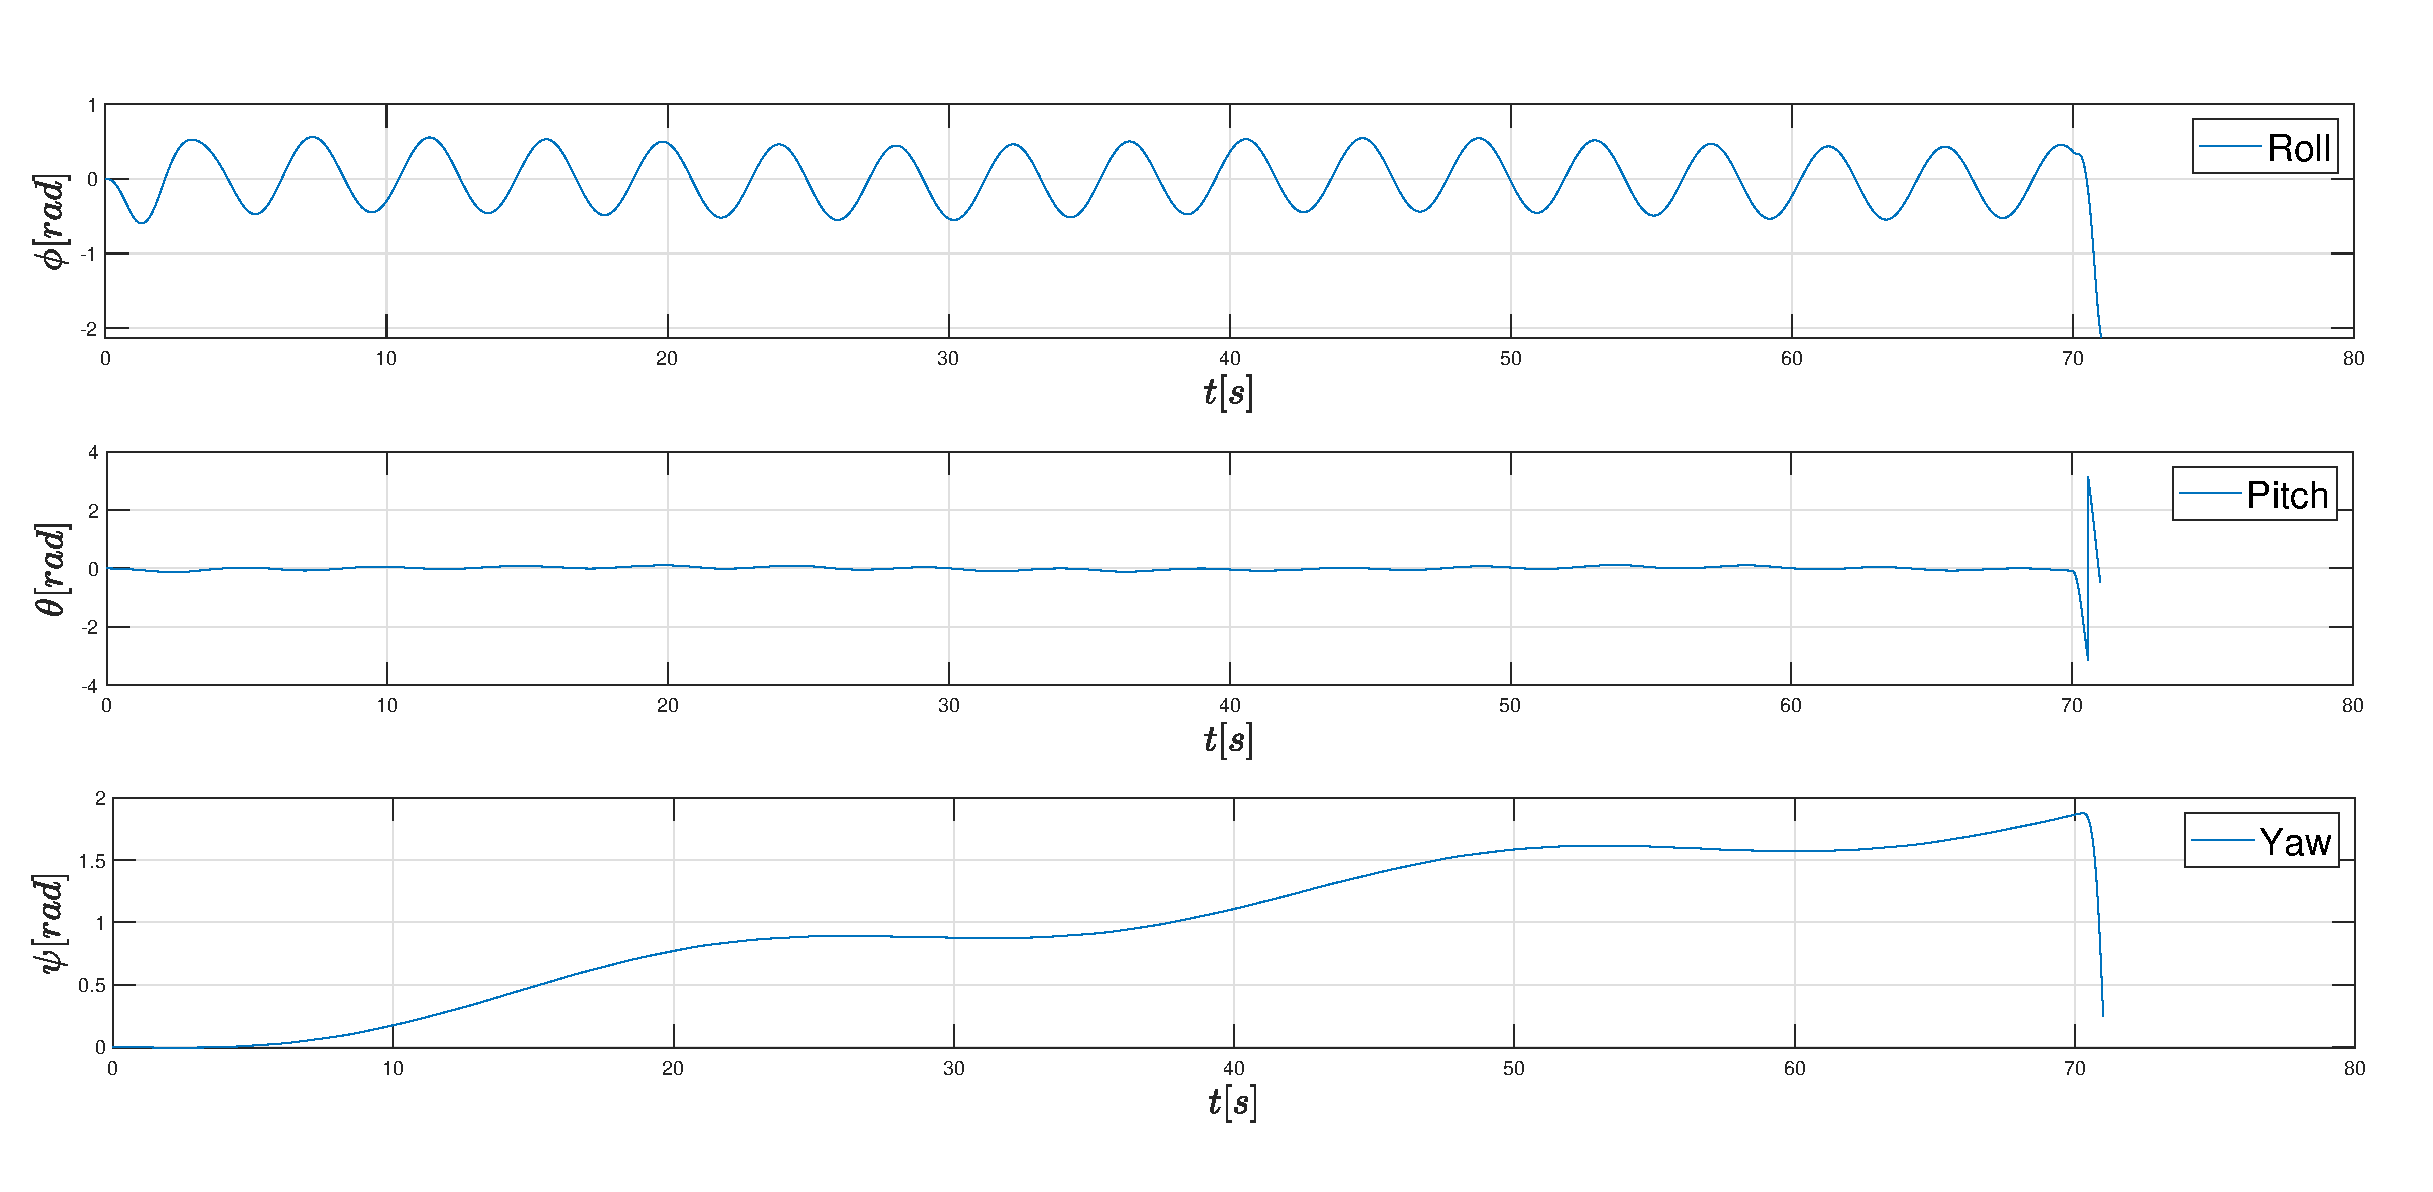
\includegraphics[scale=0.2]{figures/FL_attitude}
    \caption{Evolution of the roll, pitch and yaw angles respectively.}
    \label{fig:FL_attitude}
\end{figure}
The previous results can only be obtained if the inputs are not constrained. In fact, Figures \ref{fig:FL_angles} and \ref{fig:FL_omega} show that the value of the angle $\beta$ breaks the constraint \ref{eq:beta_constraint}. If saturations were imposed on the input signals, the system would fail to track the trajectory and diverge even in the initial phase.
\begin{figure}[H]
    \centering
    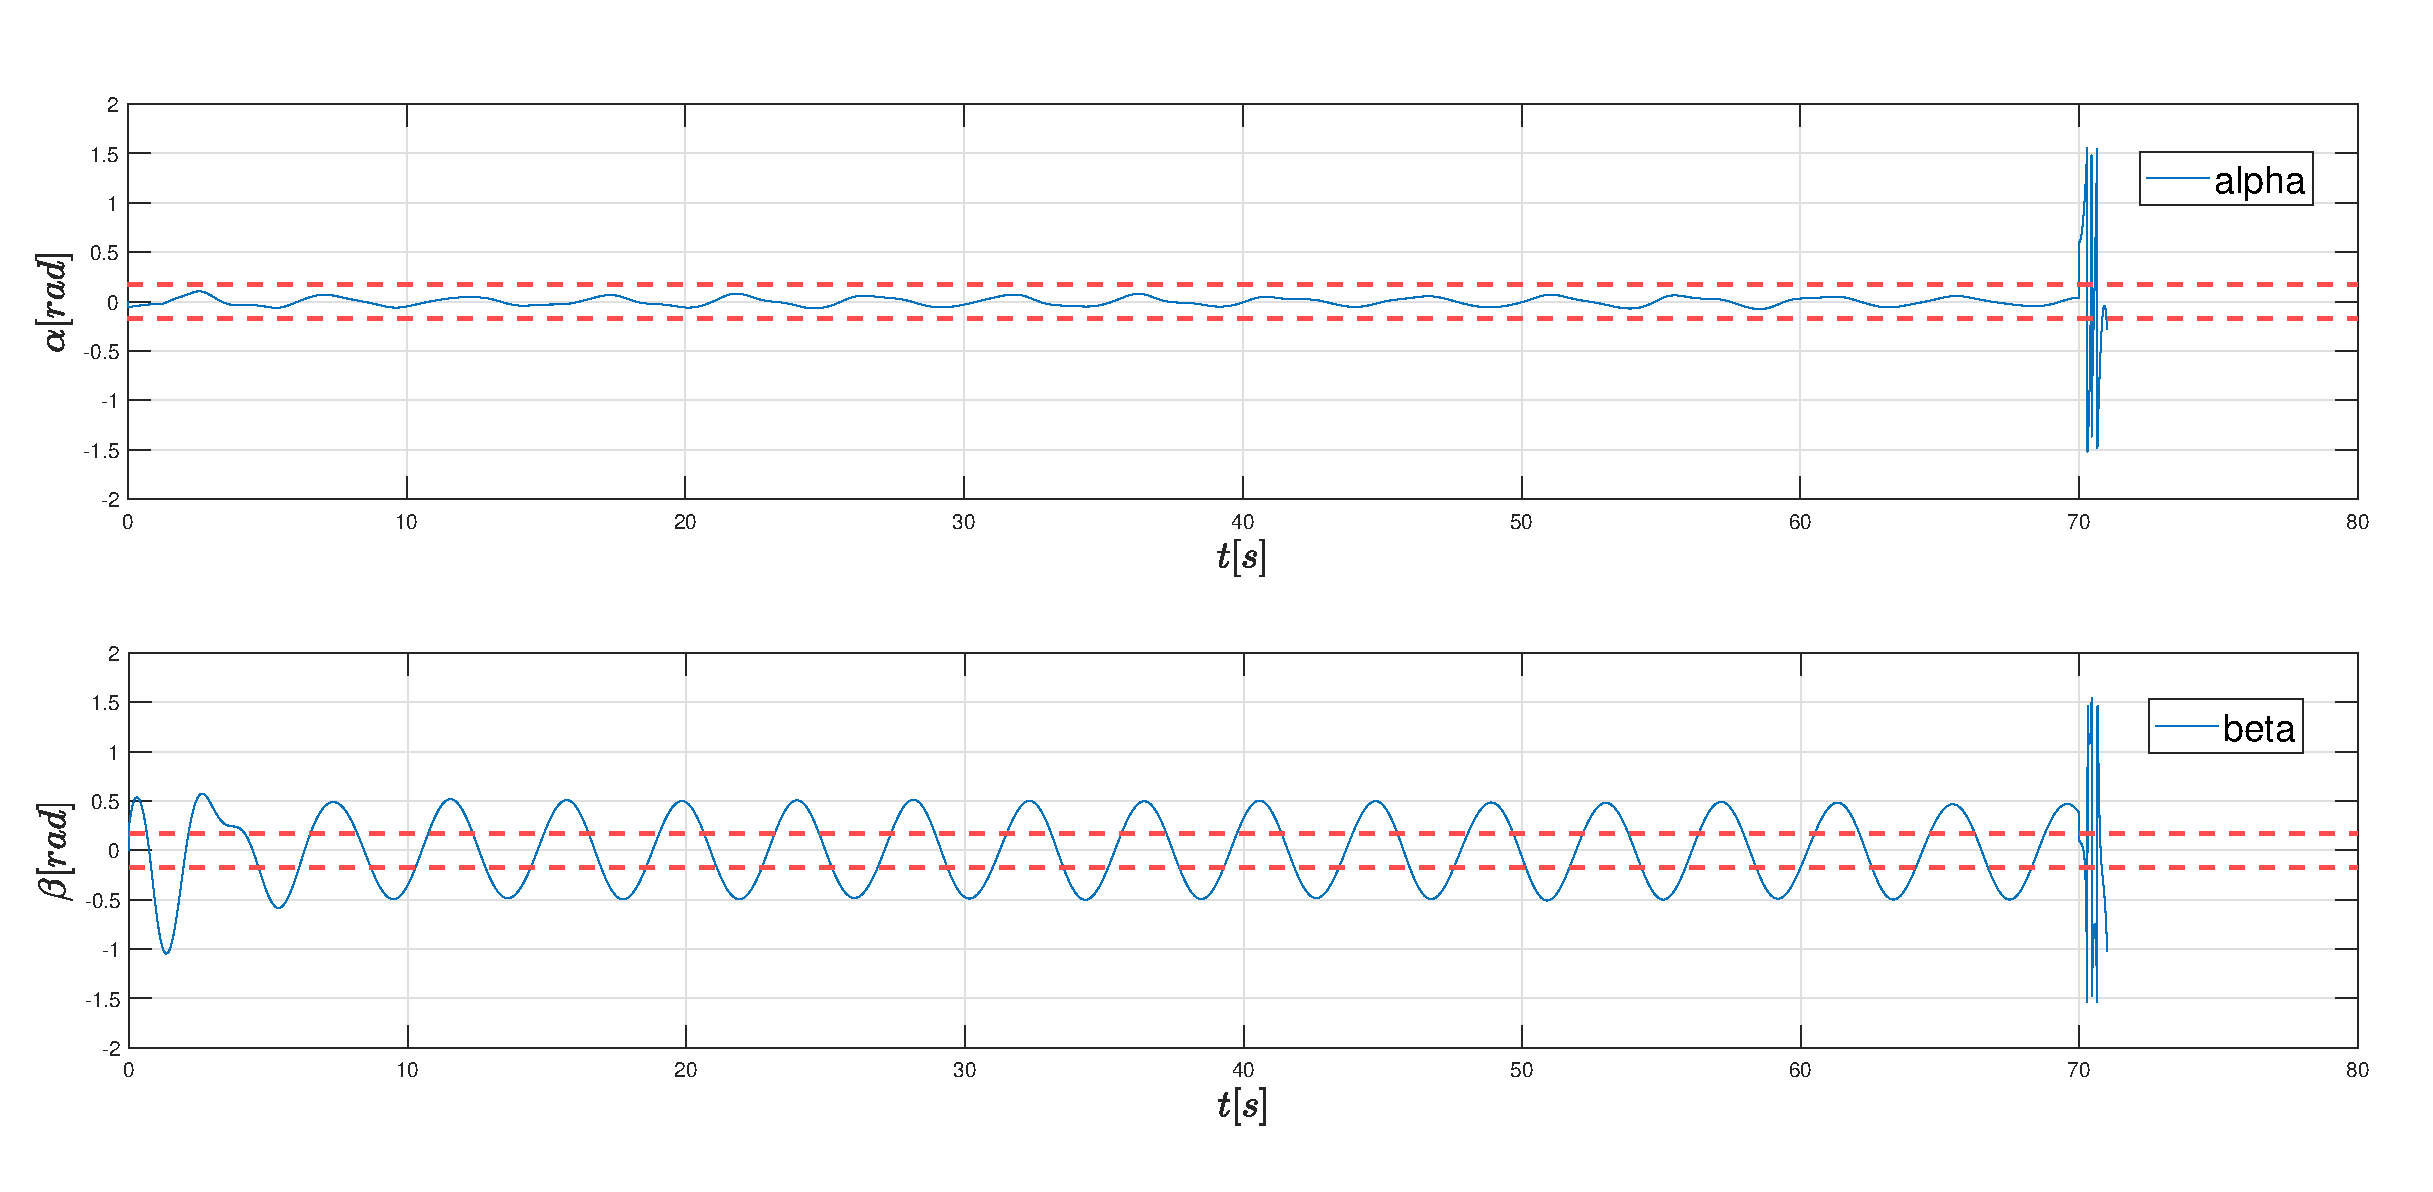
\includegraphics[scale=0.2]{figures/FL_angles}
    \caption{Angles $\alpha$ and $\beta$ of the swashplate.}
    \label{fig:FL_angles}
\end{figure}
\begin{figure}[H]
    \centering
    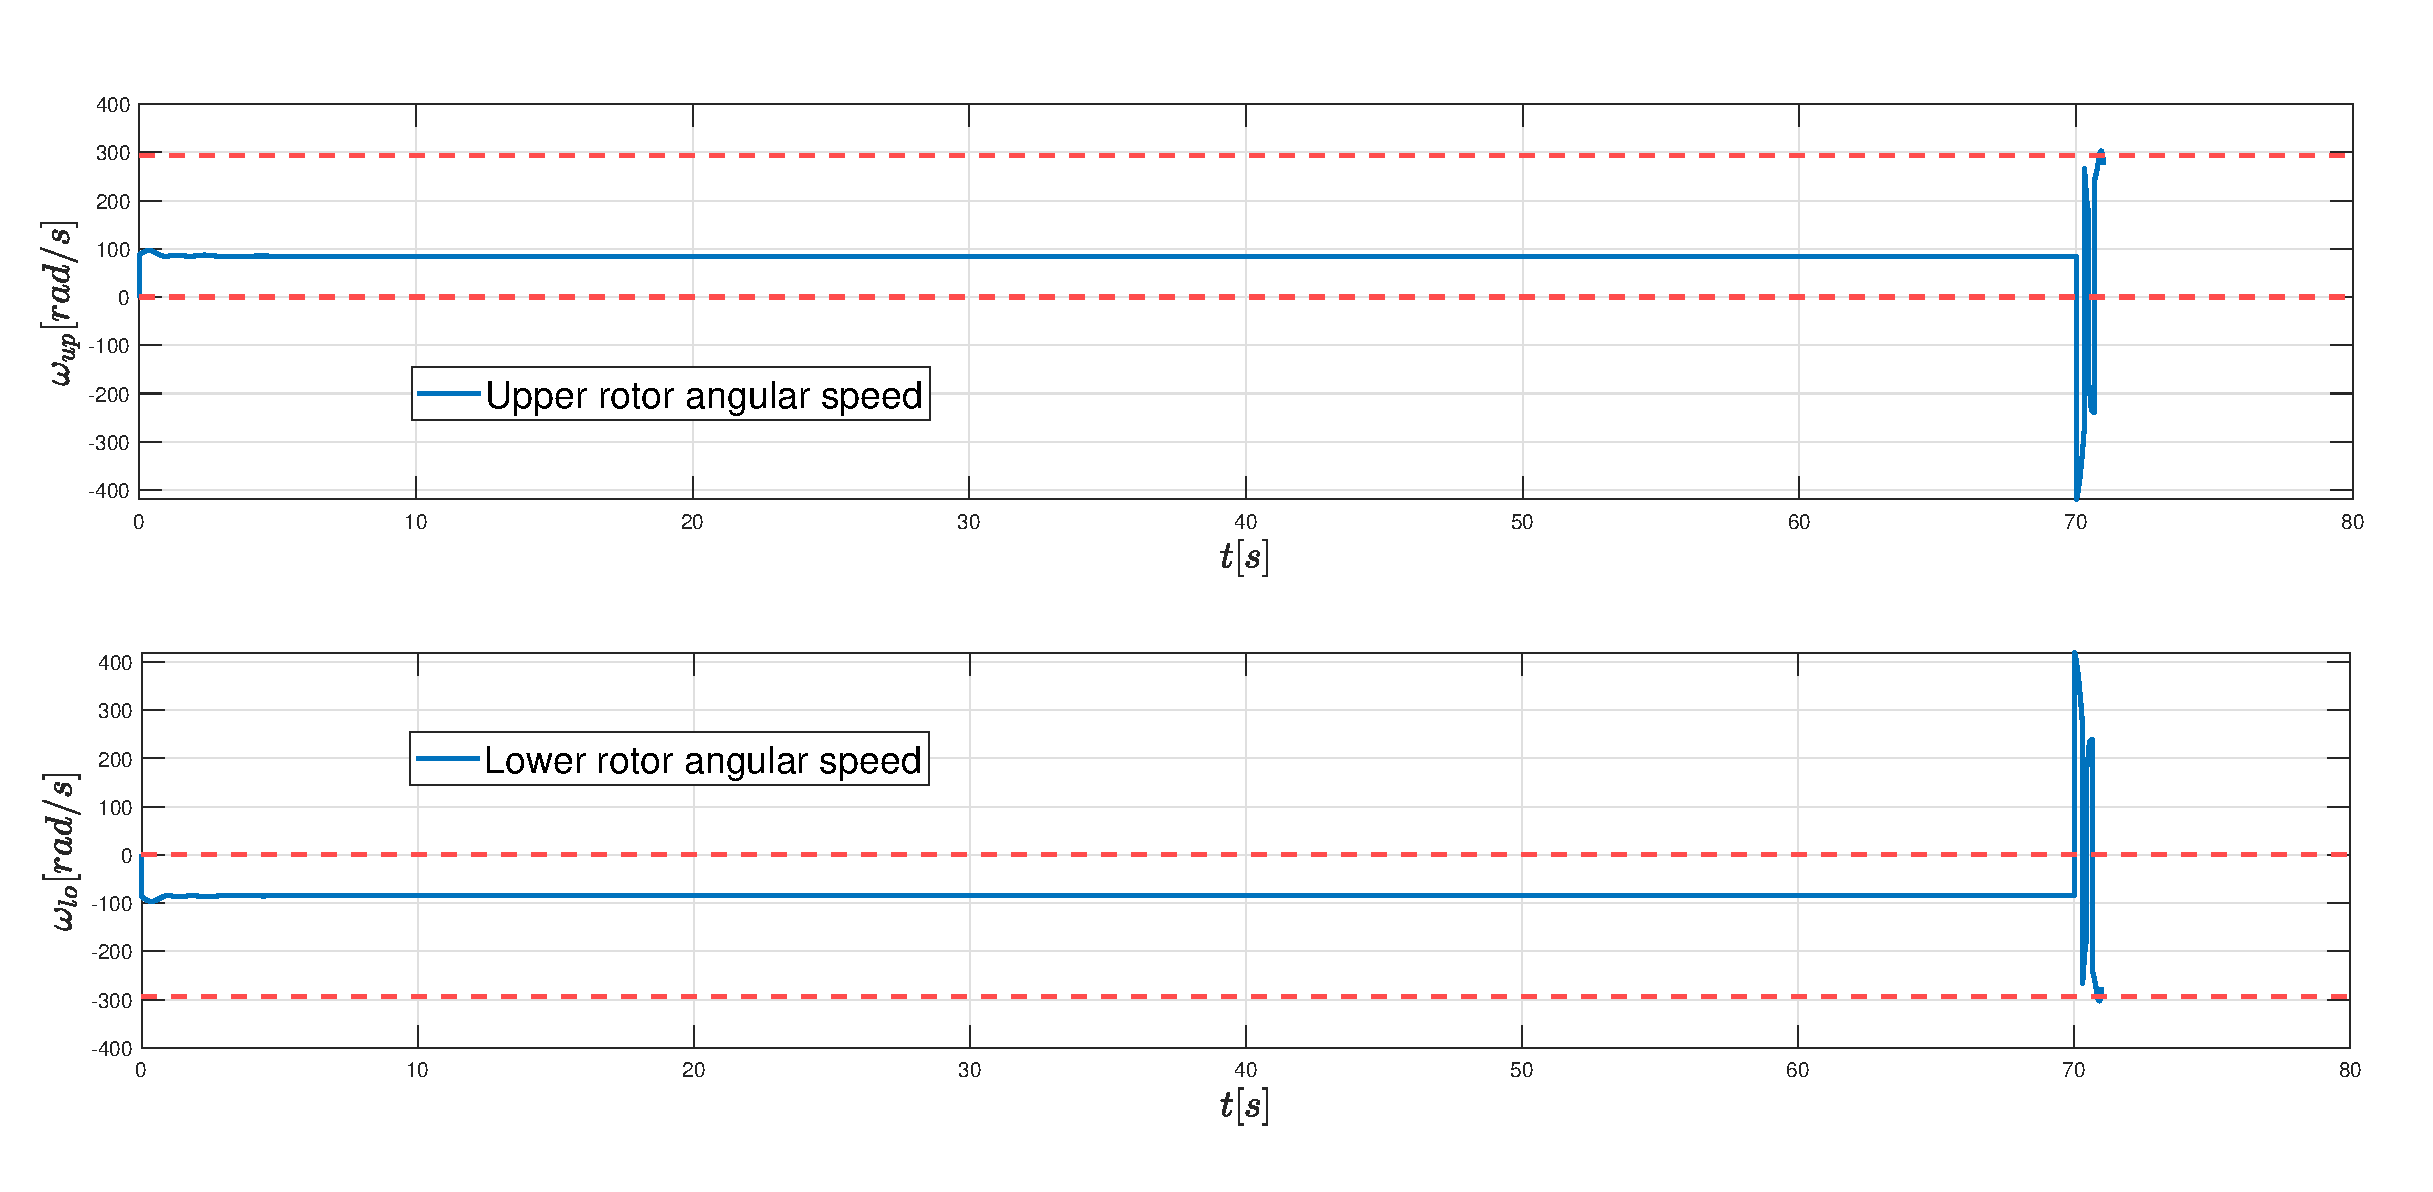
\includegraphics[scale=0.2]{figures/FL_omega}
    \caption{Angular velocities of the upper and lower rotor respectively.}
    \label{fig:FL_omega}
\end{figure}

